\documentclass[twoside]{ctexart}
\usepackage{ODE}
\title{常微分方程数值解课程报告}
\author{柏香宇, 陈晨, 孙忠豪, 张慧敏, 张梦晴, 赵权}
\date{}
\begin{document}
    \maketitle
    \tableofcontents
    \clearpage
    本次研究的方程为
    \begin{align}\label{eq:目标}
        \begin{cases}
            x'(t) = -2x(t) + \sin(\sqrt{t}), & t\in [t_{0}, t_{0}+10]\\
            x(t_{0}) = t_{0}
        \end{cases}
    \end{align}
    由常数变易法可知该方程的解析解为 
    \begin{align*}
        x(t) = \me^{-2t}\qty(\int_{t_{0}}^{t}\me^{2\tau}\sin(\sqrt{\tau})\dd{\tau} + x_{0}\me^{2t_{0}})
    \end{align*}
    这里我们取 $ t_{0}=0,\ x(t_{0})=x_{0}=1 $.

    本次实验使用的软件为 MATLAB 2021a.

    \section{显式欧拉法 (Explicit Euler Methods)}
    \subsection{介绍}
    首先给出微分方程
    \begin{align}\label{eq:一般方程}
        \begin{cases}
            x'(t)=f(x(t), t), & t\in[t_{0}, T]\\
            x(t_{0})=x_{0}.
        \end{cases}
    \end{align} 
    将 $ [t_{0}, T] $ 分为 $ n $ 个区间:
    \begin{align*}
        t_{0}=t_{0}<t_{1}<\dots<t_{n}=T,
    \end{align*}  
    对每个 $ j=1, 2, \dots, n $, 记步长 $ h_{j}=t_{j}-t_{j-1} $. 如果将 $ [t_{0}, T] $ 等分, 那么记步长为 $ h $.
    
    对方程 \eqref{eq:一般方程} 的两侧同时对 $ t $ 求积分可得:
    \begin{align*}
        x(t_{i+1})-x(t_{i})=\int_{t_{i}}^{t_{i+1}}x'(t)\dd{t} = \int_{t_{i}}^{t_{i+1}} f(x, t)\dd{t},\quad \forall i=0, 1, \dots, n-1
    \end{align*} 
    我们用 $ x_{i} $ 记 $ x(t_{i}) $ 对应的数值解, 并用左矩形公式代替右侧的积分, 就有显式欧拉法:
    \begin{align}
        x_{i+1} = x_{i} + h_{i+1}f(x_{i}, t_{i}), \quad \forall i=0, 1, \dots, n-1
    \end{align}
    对于方程 \eqref{eq:目标}, 可以构造数值格式:
    \begin{minted}[frame=none, autogobble=false]{matlab}
            x(i+1) = x(i) + h*(-2*x(i) + sin(sqrt(t(i))))
    \end{minted}

    \subsection{算法}
    \begin{algorithm}[H]
        \SetAlgoLined
        \KwIn{\mintinline{text}{f, N, StartTime, EndTime, InitialValue}}
        \KwOut{\mintinline{text}{x=x(EndTime)}}

        Initialization\;
        use \mt{StartTime}, \mt{EndTime} and \mt{N} to compute step \mt{h}\;
         \mm{t = StartTime:h:EndTime}\;
        \While{\mm{t(i)} $ \ne $ \mm{EndTime} }{
            \mm{x(i+1) = EEM(x(i), t(i))}\;
        }
        \caption{EEM}
    \end{algorithm}

    \subsection{程序}
    先写出使用显式欧拉法求解方程 \eqref{eq:一般方程} 的函数:
    {\small \inputminted{matlab}{./codes/EEM.m}}
    再使用如下脚本文件测试显式欧拉法的收敛阶:
    {\small \inputminted{matlab}{./codes/testEEM.m}}

    \subsection{输出及结论}
    得到输出结果
    \begin{center}
        \begin{tabular}{*{4}{>{$}c<{$}}}\toprule
        N_{i} & e:\abs{x_{N+1}-x(t_{N+1})}(\num{e-4}) & \text{GE}: \log_{2}(e_{i}/e_{i+1})\\\midrule
        200 & 0.3120 & - \\
        400 & 0.1547 & 1.0118 \\
        800 & 0.0770 & 1.0060 \\
        1600 & 0.0384 & 1.0030 \\
        3200 & 0.0192 & 1.0015 \\\bottomrule
    \end{tabular}
    \captionof{table}{显式欧拉法}\label{tab:EEM}
    \end{center}
            
    由 \mm{GE} 的值可知\textbf{显式欧拉法的收敛阶为 1}.

    图 \ref{fig:EEM} 为 $ N=1600 $ 时数值解的 $ t-x $ 图.
    \begin{center}
        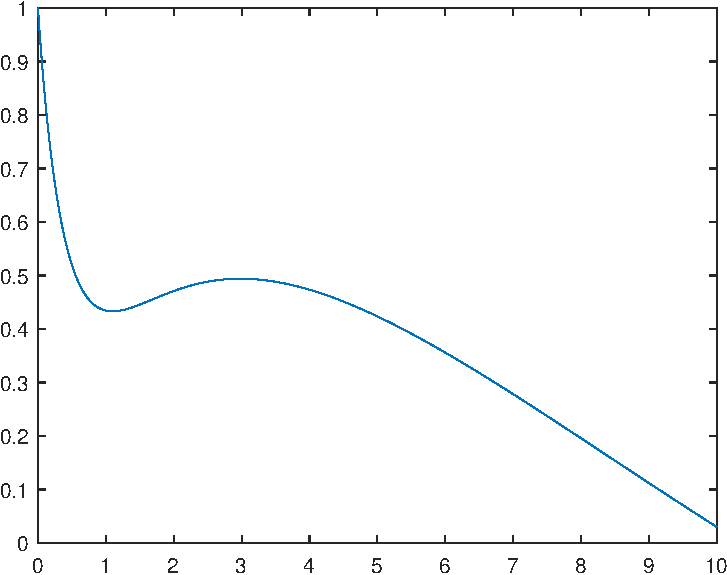
\includegraphics[width=.4\textwidth]{figs/EEM.pdf}
        \captionof{figure}{显式欧拉法, $ N=1600 $ }  \label{fig:EEM}
    \end{center}
    
    \section{隐式欧拉法 (Implicit Euler Methods)}
    \subsection{介绍}
    与显式欧拉法相同, 只是将积分 $ \int_{t_{i}}^{t_{i+1}} f(x, t)\dd{t} $ 用右矩形公式替换为 $ h_{i+1}f(x(t_{i+1}), t_{i+1}) $, 再用数值解 $ x_{i} $ 代替真解 $ x(t_{i}) $, 就可以得到隐式欧拉法:
    \begin{align}\label{eq:IEM}
        x_{i+1} = x_{i} + h_{i+1}f(x_{i+1}, t_{i+1}), \quad \forall i=0, 1, \dots, n-1
    \end{align}
    对于方程 \eqref{eq:目标}, 可以构造数值格式:
    \begin{align*}
        x_{i+1} = x_{i} + h\qty(-2x_{i+1}+\sin(\sqrt{t_{i+1}}))
    \end{align*}
    为了方便计算, 通过移项可以整理为如下的格式:
    \begin{minted}[frame=none, autogobble=false]{matlab}
            x(i+1) = 1 / (1 + 2*h) * (x(i) + h*sin(sqrt(t(i+1))))
    \end{minted}

    当然并不是所有隐式方程都可以解成 $ x_{i+1}=F(x_{i}, t_{i+1}) $ 的形式, 那么可以使用 Newton 迭代法来求 $ x_{i+1} $ 的近似值. 要在方程 \eqref{eq:IEM} 中解出 $ x_{i+1} $, 即求非线性方程
    \begin{align*}
        g(y)=y - x_{i} - hf(y, t_{i+1})=0
    \end{align*}
    的根, 其中 $ x_{i} $ 与 $ t_{i+1} $ 均为已知, 取 $ y=x_{i} $ 为迭代初值 $ y_{0} $, 按
    \begin{align*}
        y_{j+1} = y_{j}-\frac{g(y_{j})}{g'(y_{j})}=y_{j}-\frac{y_{j}-hf(y_{j}, t_{i+1})-x_{i}}{g'(y_{j})},\quad \forall j\in \N
    \end{align*} 
    来对 $ g(y)=0 $ 的根进行迭代, 一般进行 10 次即可满足需求. 于是对于方程 \eqref{eq:目标} 只要求出 $ g'(y) $ 即可, 而显然有 $ g'(y)=1+h $. 
    
    下面将给出两种方法的程序与收敛阶的验证, 并进行对比.
 
    \subsection{算法}
    \begin{algorithm}[H]
        \KwIn{\mintinline{text}{f, N, StartTime, EndTime, InitialValue}}
        \KwOut{\mintinline{text}{x=x(EndTime)}}

        Initialization\;
        use \mt{StartTime}, \mt{EndTime} and \mt{N} to compute step \mt{h}\;
        \mm{t =StartTime:h:EndTime}\;
        \While{\mm{t(i)} $ \ne $ \mm{EndTime} }{
            \mm{x(i+1) = F(x(i), t(i+1))};
        }
        \caption{显式解出 $ x_{i+1}=F(x_{i}, t_{i+1}) $ }
    \end{algorithm}

    \begin{algorithm}[H]
        \KwIn{\mintinline{text}{f, N, StartTime, EndTime, InitialValue}}
        \KwOut{\mintinline{text}{x=x(EndTime)}}

        Initialization\;
        use \mt{StartTime}, \mt{EndTime} and \mt{N} to compute step \mt{h}\;
        \mm{t =StartTime:h:EndTime}\;
        compute \mm{dg}\;
        \While{\mm{t(i)} $ \ne $ \mm{EndTime} }{
            \mm{y = x(i)}\;
            \Repeat(Newton's Method){\mm{|y(j+1)-y(j)|<ErrorValue}, 10 times of iteration are enough often.}{\mm{y(j+1) = y(j) - g(y_{j})/dg(y_{j})}}
            \mm{x(i+1) = y}\;
        }
        \caption{使用牛顿迭代法求 $ x_{i+1} $ }
    \end{algorithm}

    \subsection{程序}
    由于隐式欧拉法需要解方程来求得 \mm{x(i)} 的下一步 \mm{x(i+1)}, 而计算机不擅长这个工作, 所以函数 \mt{IEM.m} 只为方程 \eqref{eq:目标} 设计, 函数如下
    
    {\small\inputminted{matlab}{./codes/IEM.m}\captionof{code}{显式解出 $ x_{i+1}=F(x_{i}, t_{i+1}) $ }}

    {\small\inputminted{matlab}{./codes/IEMNT.m}\captionof{code}{使用牛顿迭代法求 $ x_{i+1} $ }}

    并且使用如下脚本测试收敛阶:

    {\small\inputminted{matlab}{./codes/testIEM.m}}

    \subsection{输出及结论}
    沿用表 \ref{tab:EEM} 的记号, 将输出整理为表格可得
    \begin{center}
        \begin{tabular}{*{6}{>{$}c<{$}}}\toprule
            N_{i} & \abs{x_{i}-y_{i}} (\num{e-14}) & e_{x} (\num{e-4}) & e_{y} (\num{e-4}) & \text{GE}_{x} & \text{GE}_{y}\\\midrule
            200 & 0.2717 & 0.3017 & 0.3017 & - & - \\
            400 & 0.0059 & 0.1521 & 0.1521 & 0.9877 & 0.9877 \\
            800 & 0.0284 & 0.0764 & 0.0764 & 0.9939 & 0.9939 \\
            1600 & 0.0337 & 0.0383 & 0.0383 & 0.9970 & 0.9970 \\
            3200 & 0.1481 & 0.0192 & 0.0192 & 0.9985 & 0.9985 \\\bottomrule
        \end{tabular}
        \captionof{table}{IEM}\label{IEM}
    \end{center}
    
    可见即使用牛顿法进行迭代出的近似值与显式解出 $ x_{i+1} $ 得到的值的差距极小, 故在解一般的隐式方程的时候, 可以使用牛顿法来求解, 而不用担心误差过大. 同样从 \mm{GE} 的值可以看出\textbf{隐式欧拉法的收敛阶为 1}.
    
    图 \ref{fig:IEM} 为使用牛顿法迭代法 $ N = 1600 $  时数值解的 $ t-x $  图.
    \begin{center}
        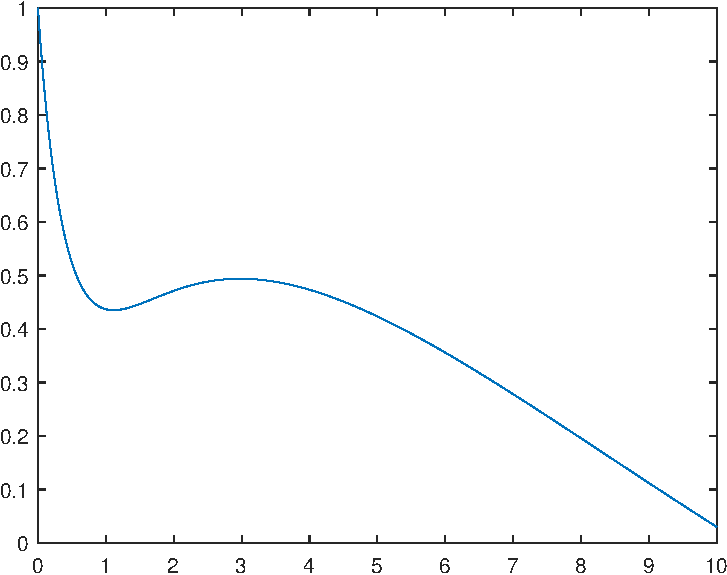
\includegraphics[width=.4\textwidth]{figs/IEMNT.pdf}
        \captionof{figure}{隐式欧拉法, $ N=1600 $}  \label{fig:IEM}
    \end{center}

    \section{RK 法 (Runge-Kutta Methods)}
    \subsection{介绍}
    RK 法是一个一步法, 包含了很多级 (stage). 显式欧拉法 EEM 与 RK 法都是用一条经过 $ (t_{n}, x(t_{n})) $ 的直线 $ \ell_{n} $ 来决定 $ t_{n+1} $ 点的值, 关键是这条直线的斜率应该如何选择才能让 $ t_{n+1} $ 点的值更接近真实的值. 在 EEM 中仅用了 $ (t_{n}, x(t_{n})) $ 点的斜率 $ f(x(t_{n}), t_{n}) $ 来作为 $ \ell_{n} $ 的斜率. 而 $ s $ 级 RK 法 ($ s $-stage RK method) 选取 $ [t_{n}, t_{n+1}] $ 中的 $ s $ 个点的斜率的近似值进行加权平均来作为 $ \ell_{n} $ 的斜率来提高精度, 它通常被写为 
    \begin{align}\label{eq:RKi+1}
        x_{n+1} = x_{n} + h\Sum{i=1}{s}b_{i}k_{i}
    \end{align}
    其中 $ \qty{k_{i}} $ 是各斜率的近似值:
    \begin{align}
        k_{i} & := f\qty(x(t_{n}+c_{i}h), t_{n}+c_{i}h)\notag\\
        & \approx f\qty(x_{n}+h\Sum{j=1}{s}a_{i, j}k_{j}, t_{n}+c_{i}h), \quad i=1, 2, \dots, s,\label{eq:RK}
    \end{align} 
    而又易证
    \begin{align*}
        c_{i} = \Sum{j=1}{s}a_{i, j},\quad i = 1, 2, \dots, s,
    \end{align*}
    于是只要给定了级数 $ s $, 那么一个 $ s $-级的 RK 法就可以用一个 Butcher 表 \ref{eq:fullbutcher} 表示出来
    
    \begin{align*}
        \begin{NiceArray}{c|*{4}{c}}
            c_{1} & a_{1, 1} & a_{1, 2} & \cdots & a_{1, s}\\
            c_{2} & a_{2, 1} & a_{2, 2} & \cdots & a_{2, s}\\
            \vdots & \vdots & \vdots & \ddots & \vdots\\
            c_{s} & a_{s, 1} & a_{s, 2} & \cdots & a_{s, s}\\\hline
            & b_{1} & b_{2} & \cdots & b_{s} 
        \end{NiceArray}
    \end{align*}
    \captionof{table}{Butcher 表}\label{eq:fullbutcher}
    可以将它简记为 $ \begin{NiceArray}{c|c}
        c & A\\\hline
        & b^{\top}
    \end{NiceArray} $, 于是我们可以看到, 显式欧拉法 EEM 是一个一级的 RK 法, 即
    \begin{align*}
        \begin{cases}
        x_{n+1} = x_{n} + hk\\
        k = f(x_{n}, t_{n})            
        \end{cases}
    \end{align*}
    如果与 Buther 表对应, 那么 $ A = \qty(a_{11})=\qty(0), b = \qty(1), c = \qty(0) $. 特别地, 如果
    \begin{align*}
        A = \begin{pNiceArray}{ccc}
            0 & \Cdots & 0\\
            \Block{2-2}<\Large>{*} & \Ddots & \Vdots\\
            & & 0
        \end{pNiceArray}
    \end{align*}
    那么这个方法是 $ s $ 级 ERK 法 (Explicit Runge-Kutta Methods). 这次报告以经典的 3 级 3 阶 RK 法与 4 级 4 阶 RK 法为例进行编程, 它们的 Butcher 表分别为
    \begin{align*}
        \begin{NiceArray}{c|ccc}
            0 & & & \\
            \frac{1}{2} & \frac{1}{2} & & \\
            1 & -1 & 2 &  \\\hline
            & \frac{1}{6} & \frac{2}{3} & \frac{1}{6}
        \end{NiceArray}\qquad
        \begin{NiceArray}{c|cccc}
            0 & & & & \\
            \frac{1}{2} & \frac{1}{2} & & & \\
            \frac{1}{2} & 0 & \frac{1}{2} & & \\
            1 & 0 & 0 & 1 & \\\hline
             & \frac{1}{6} & \frac{1}{3} & \frac{1}{3} & \frac{1}{6}
        \end{NiceArray}
    \end{align*}

    \subsection{算法}
    \begin{algorithm}[H]
        \KwIn{\mintinline{text}{f, N, StartTime, EndTime, InitialValue, Index}}
        \KwOut{\mintinline{text}{x=x(EndTime)}}

        Initialization\;
        use \mt{StartTime}, \mt{EndTime} and \mt{N} to compute step \mt{Step}\;
        use \mt{Index} to get matrix \mt{A, b, c}\;
         \mm{Time =StartTime:h:EndTime}\;
        \While{\mm{t(i)} $ \ne $ \mm{EndTime} }{
            \For{every row \mm{A(j)} in \mm{A}}{
                compute \mm{K(j)} with eq \eqref{eq:RK}\; 
            }
            compute \mm{x(i+1) = x(i) + Step * b' * k}\;
        }
        \caption{ERK 法}
    \end{algorithm}

    \subsection{程序}

    先编写函数 \mt{Method.m} 来存储 3 级与 4 级 RK 法的 Butcher 表的矩阵 $ A, b, c $:
    {\small\inputminted{matlab}{./codes/Method.m}}

    再编写函数 \mt{ERK.m} 来使用 \mt{Index} 作为 RK 法的索引:
    {\small\inputminted{matlab}{./codes/ERK.m}}

    最后编写函数 \mt{testERK.m} 来测试两种 RK 法的收敛阶:
    {\small\inputminted{matlab}{./codes/testERK.m}}

    \subsection{输出及结论}

    沿用表 \ref{tab:EEM} 的记号, 将输出整理为表格可得
    \begin{center}
        \begin{tabular}{*{5}{>{$}c<{$}}}\toprule
            N_{i} & e_{x} (\num{e-7}) & e_{y} (\num{e-9}) & \text{GE}_{x} & \text{GE}_{y}\\\midrule
            200 & 0.2652 & 0.7428 & - & - \\
            400 & 0.0326 & 0.0454 & 3.0259 & 4.0333 \\
            800 & 0.0040 & 0.0027 & 3.0130 & 4.0492 \\
            1600 & 0.0005 & 0.0001 & 3.0061 & 4.2270 \\
            3200 & 0.0001 & 0.0000 & 3.0018 & 7.9296 \\\bottomrule
        \end{tabular}
        \captionof{table}{ERK}\label{ERK}
    \end{center}

    可见 3 级的 RK 法精度比 4 级 RK 法要低, 但是误差远小于欧拉法, 这说明增加中间值对于 1 步法来说是有必要的, 同时由 \mt{GEx} 与 \mt{GEy} 的值可以看出 \textbf{Kutta 3 级 RK 法的收敛阶为 3}, \textbf{经典 4 级 RK 法的收敛阶为 4}. 

    图 \ref{fig:ERK} 为 $ N=3200 $ 时经典 4 级 RK 法的数值解的 $ t-x $ 图. 
    \begin{center}
        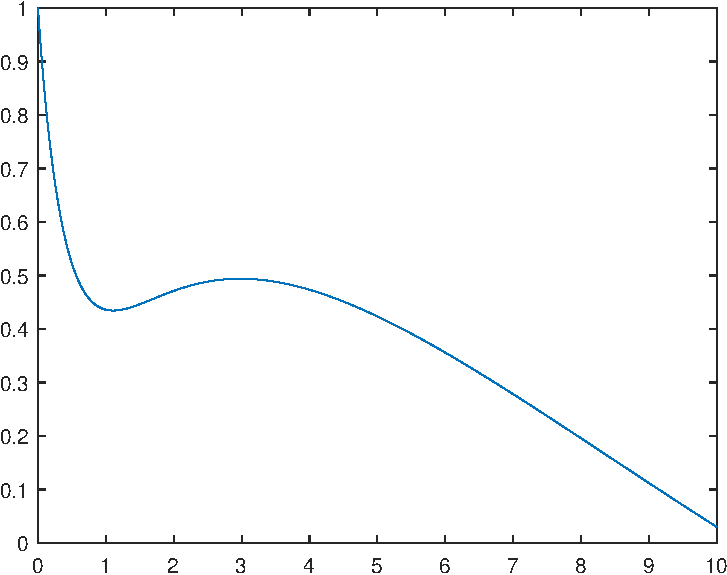
\includegraphics[width=.4\textwidth]{figs/ERK.pdf}
        \captionof{figure}{RK Methods}\label{fig:ERK}
    \end{center}
\end{document}